\chapter{Apoio à Docência}
\label{cap: apoioDocencia}
Neste capítulo, apresentaremos os principais recursos físicos e estruturais da \ac{GPF}, disponíveis aos docentes para melhor desempenharem suas atividades.

\section{Sala dos Professores}
\setlength\intextsep{0pt}
\begin{wrapfigure}[9]{r}{0.5\textwidth}
    \centering
    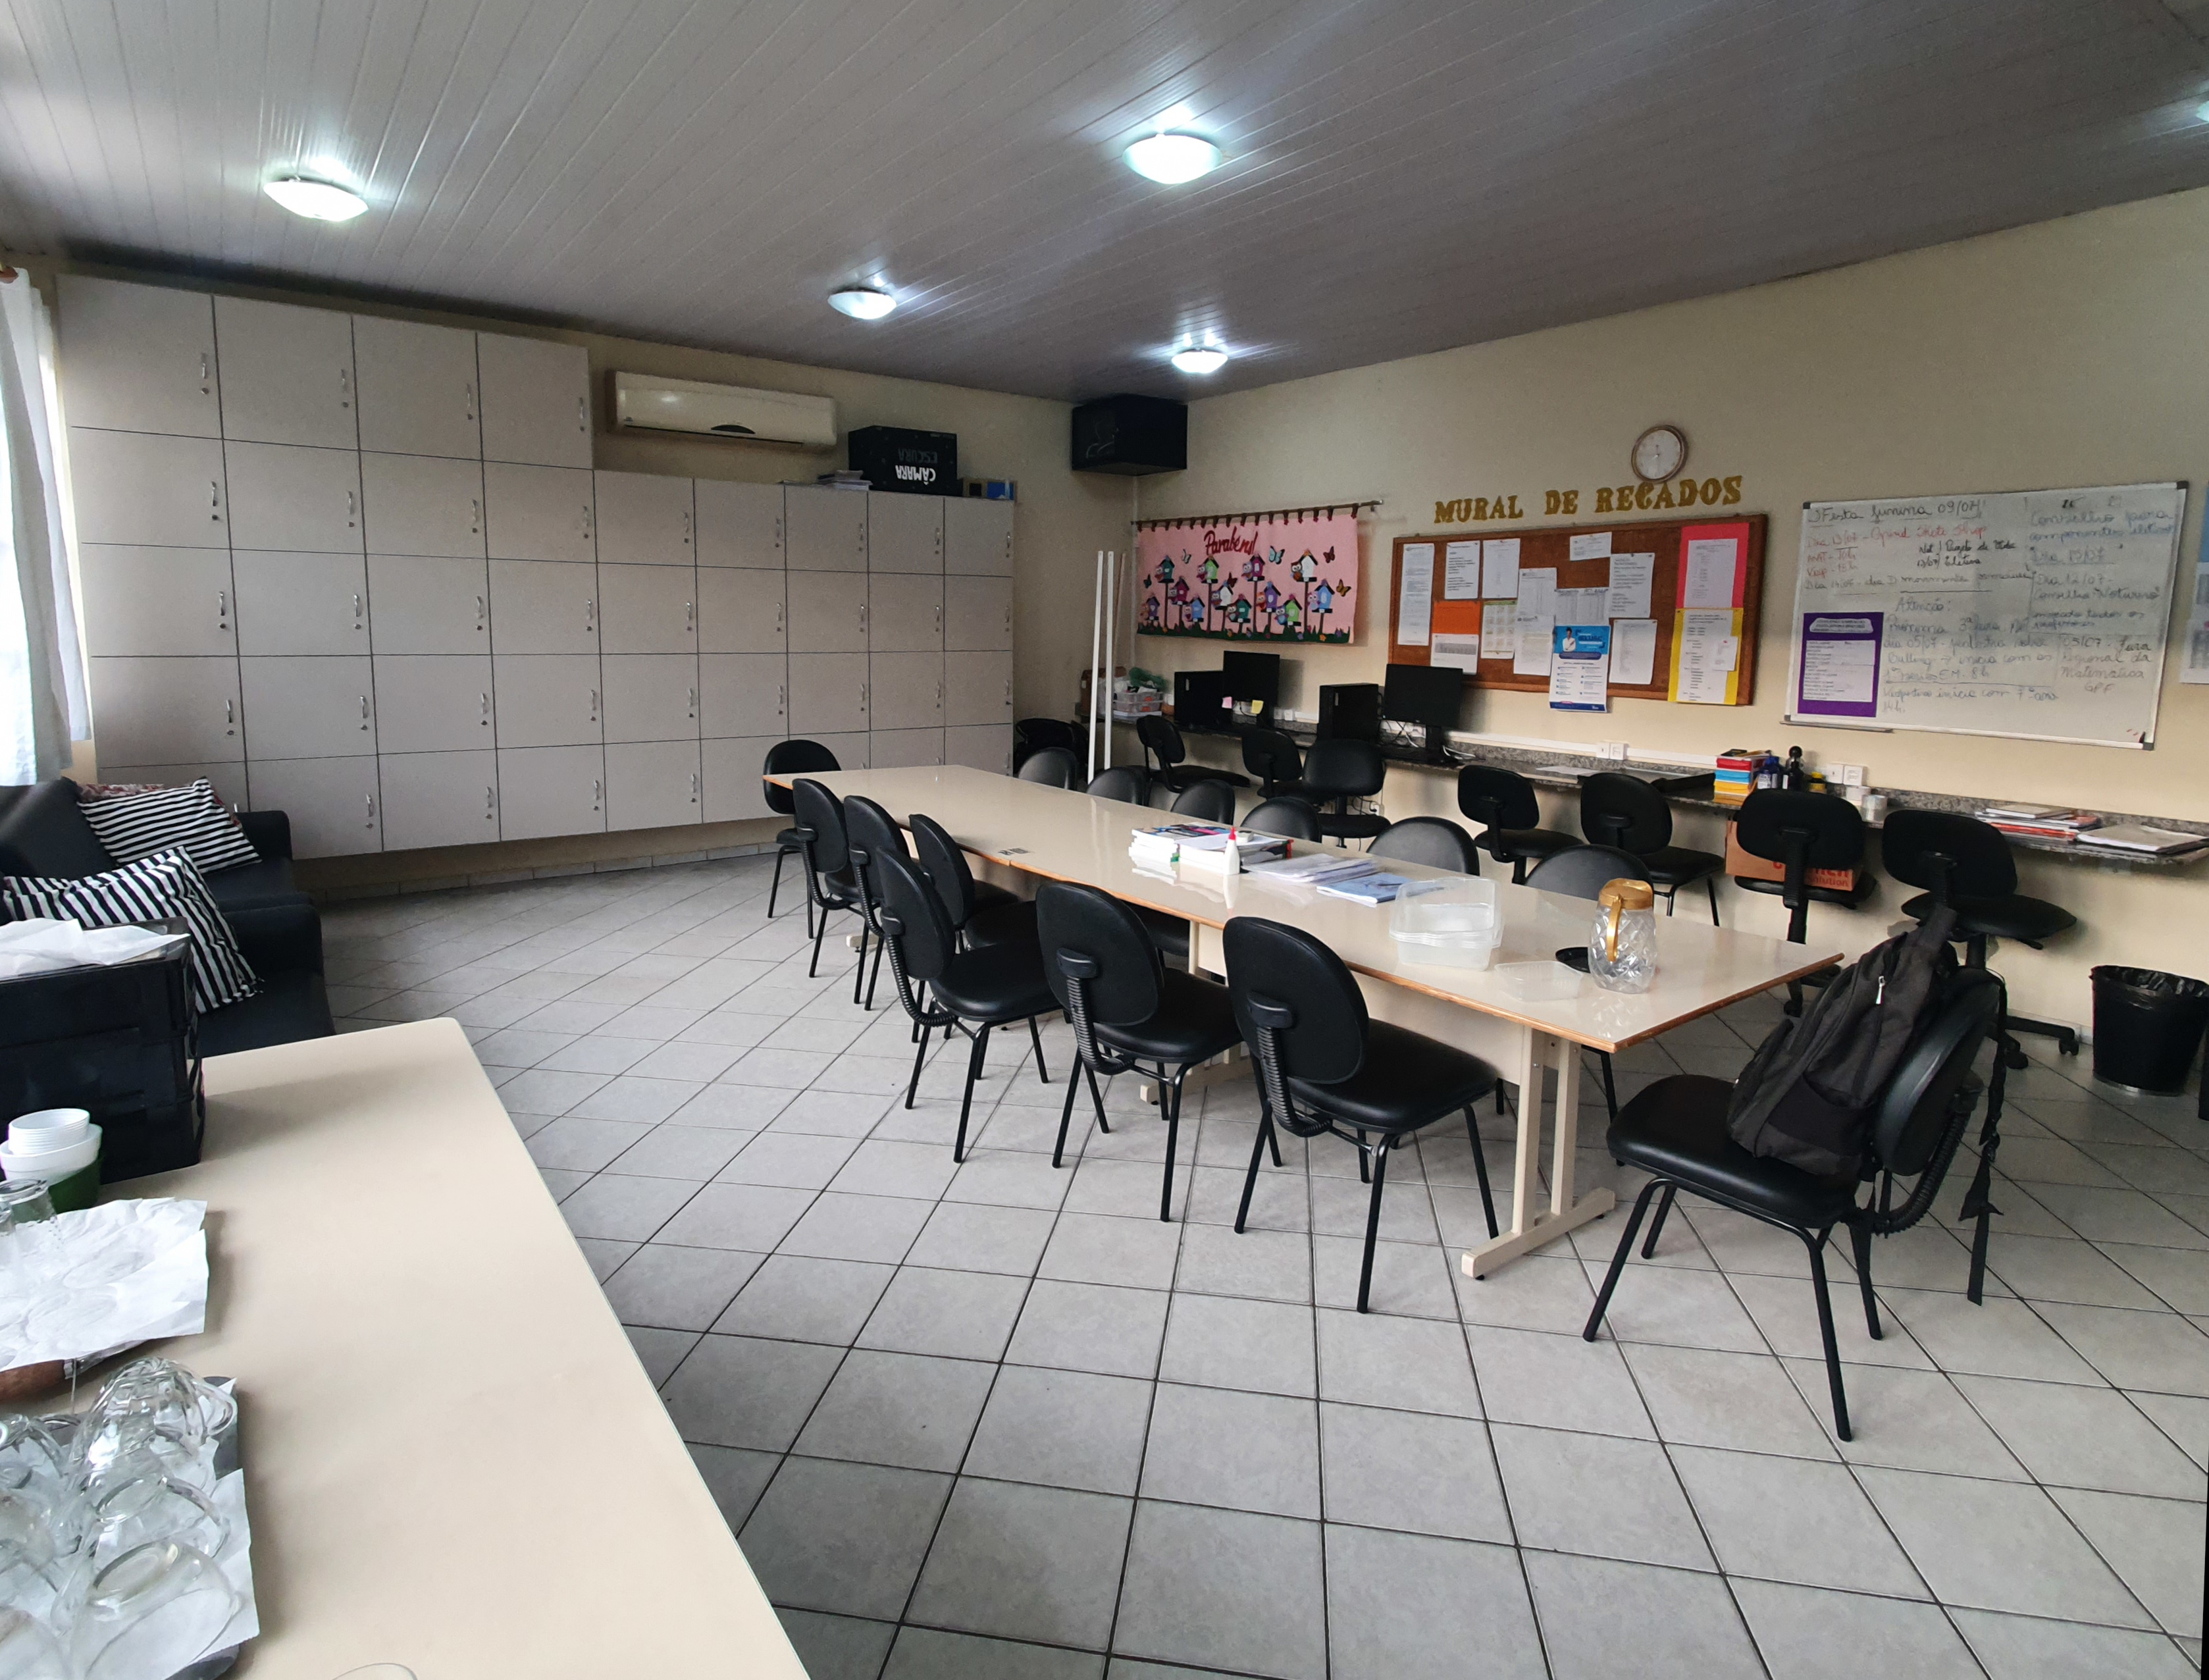
\includegraphics[width=.45\textwidth]{03-elementos/03.2_textual/03.2.1_fig/sala-de-profs01.jpg}
    
    \label{fig:salaDosProfs}
    \caption{Sala dos Professores}    
\end{wrapfigure}
Bem espaçosa a Sala dos Professores possui: geladeira, microondas, ar-condicionado e um purificador de água. É equipada com dois desktops conectados à internet. Cada professor tem um espaço nos armários, e é nele que fica guardado o \emph{Data-Show} para uso em aulas diferenciadas.

\section{Laboratório}
As aulas experimentais podem ser conduzidas no Laboratório, preparado para atender as disciplinas de Física, Química e Biologia. Comporta cerca de 40 alunos, e é composto por duas grandes bancadas e alguns armários. Infelizmente no momento em que este relatório foi escrito, encontrava-se interditado devido à alocação dos materiais para montar a festa junina. Dessa forma, a entrada ao laboratório estava restrita apenas para a equipe gestora.

\section{Laboratório de informática}
\setlength\intextsep{0pt}
\begin{wrapfigure}[9]{l}{0.5\textwidth}
    \centering
    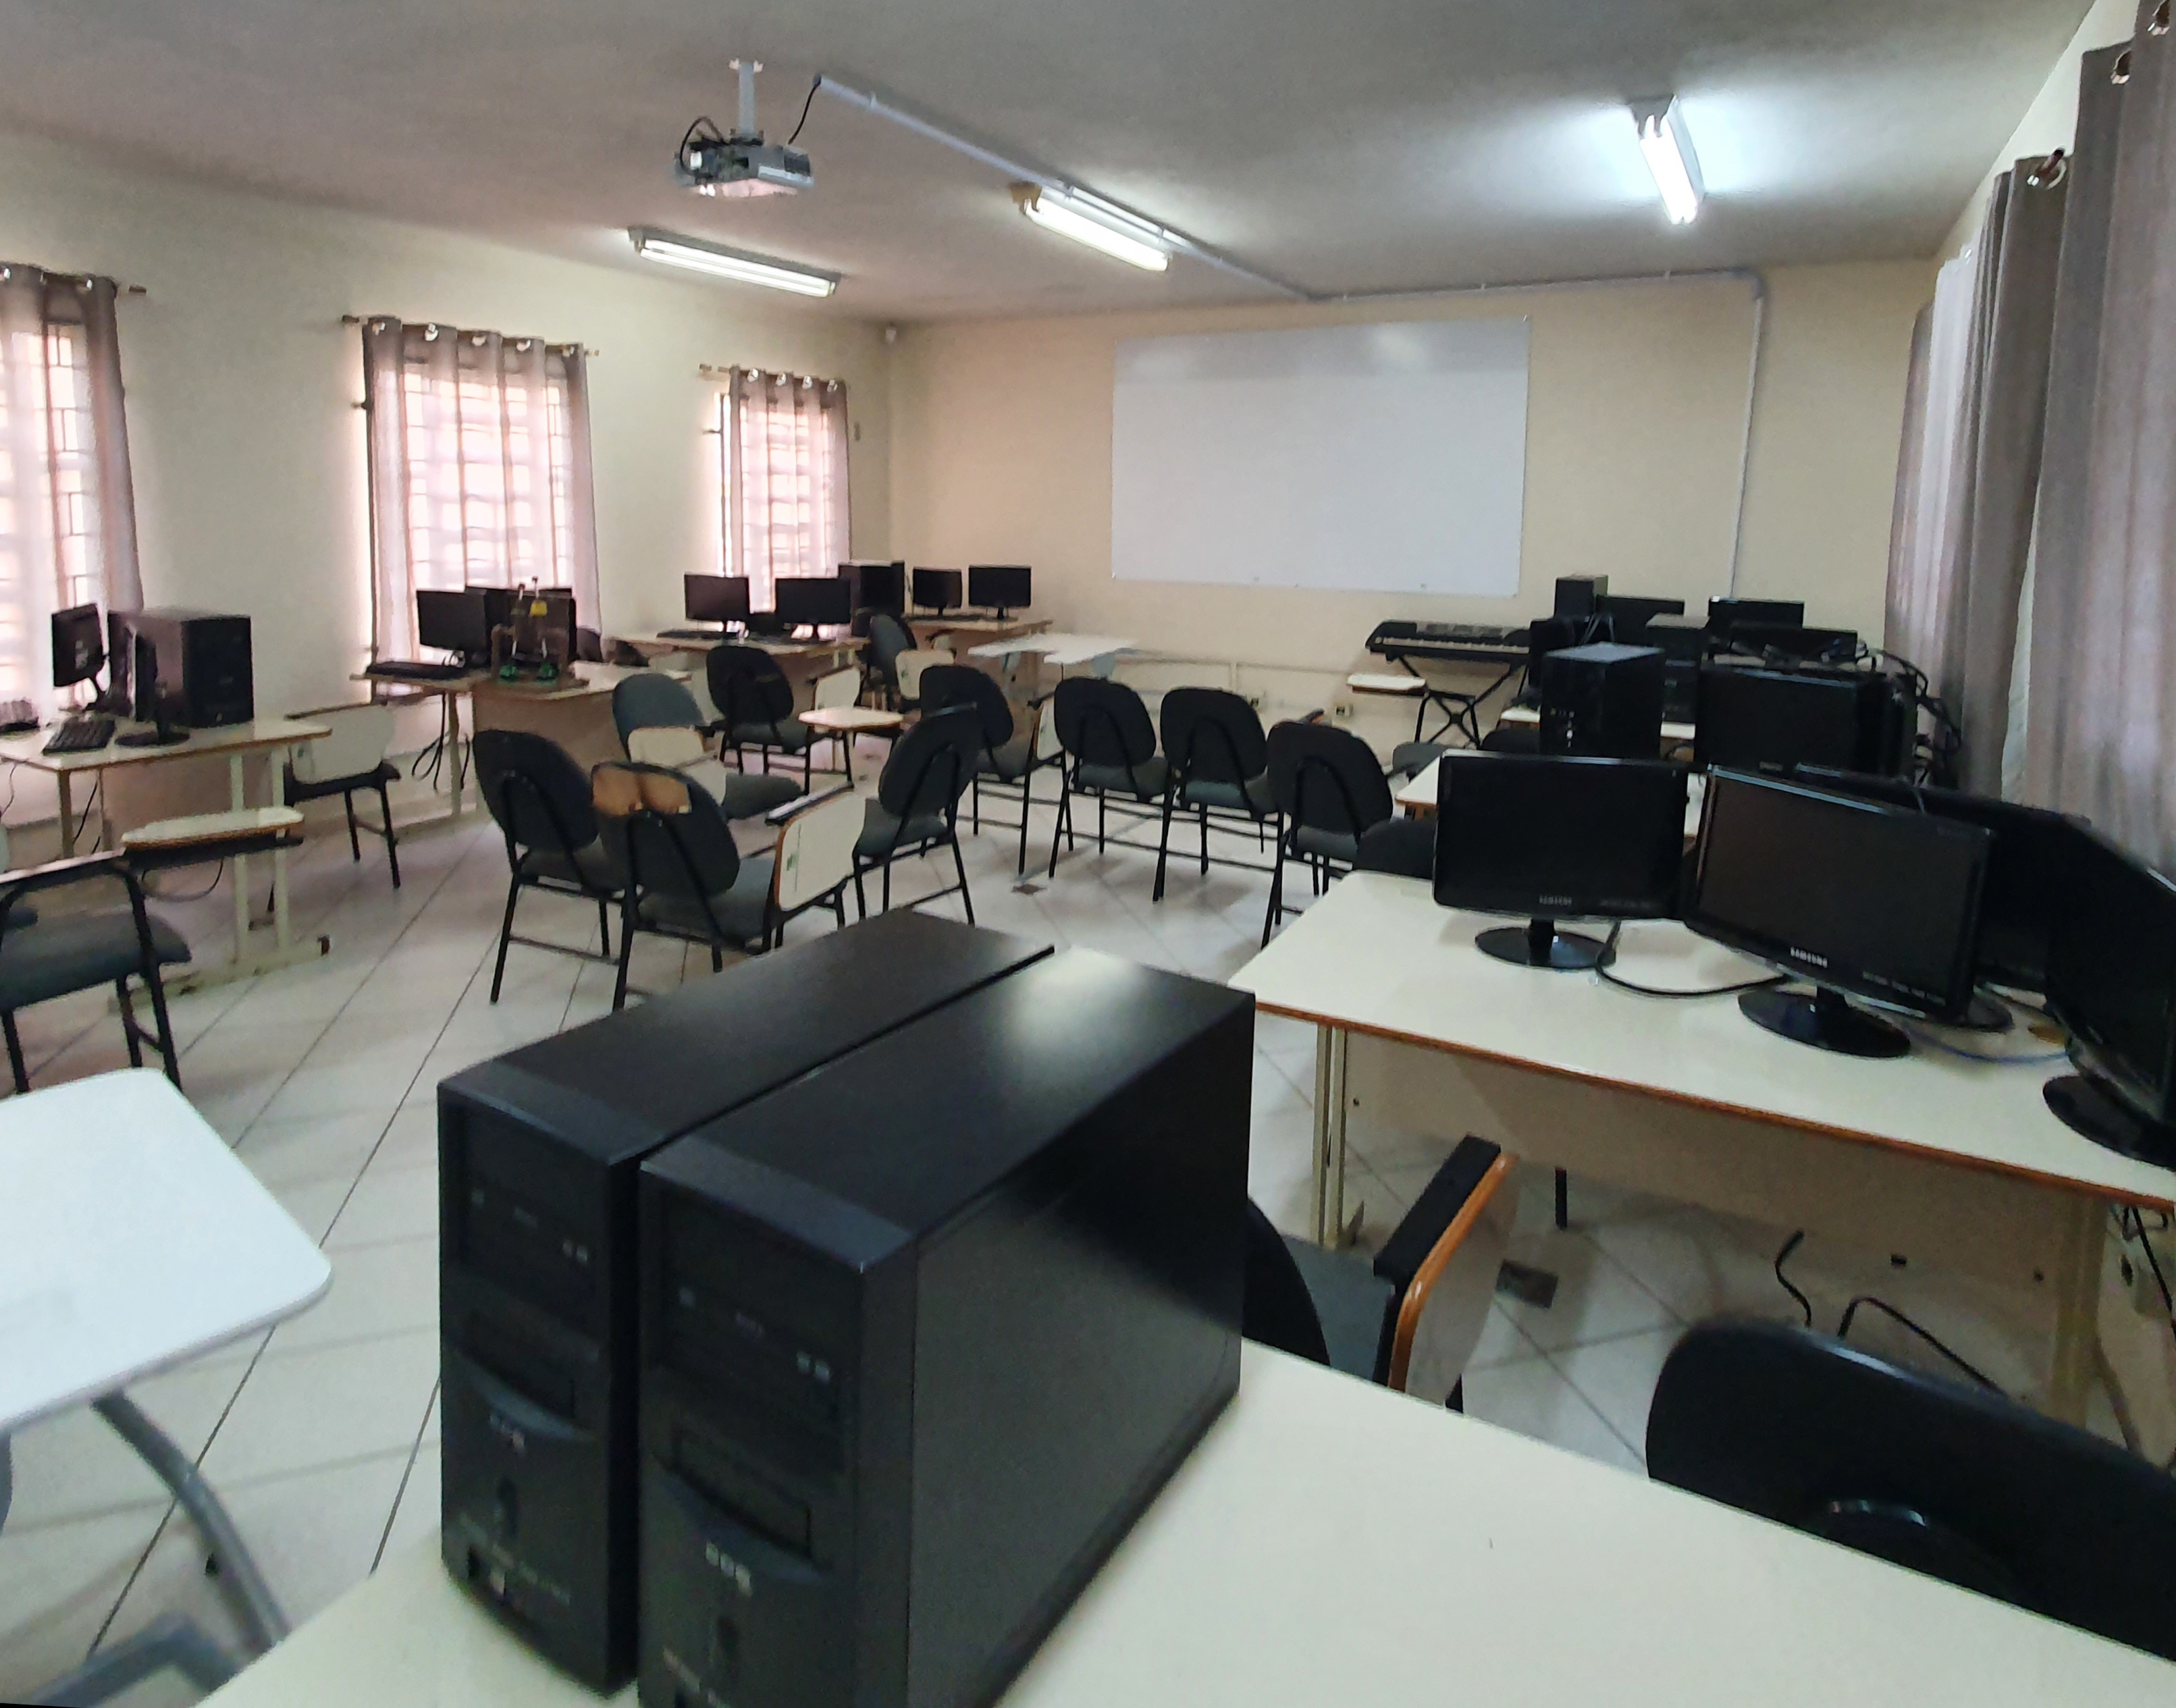
\includegraphics[width=.45\textwidth]{03-elementos/03.2_textual/03.2.1_fig/sala-de-informatica02.jpg} 
    \caption{Laboratório de informática}
    \label{fig:salaDeInformatica}  
\end{wrapfigure}
O Laboratório de Informática é composto por 9 desktops e 19 monitores com acesso à internet, tem capacidade para atender até 19 alunos em virtude da quantidade de dispositivos. Possui ainda uma Lousa Melamínica ($350\times 120$)\cm\; e retroprojetor.

\section{Salas de aula}
As Salas de Aulas são planejadas para comportar em média 30 alunos. Boa parte das salas possuem ar-condicionados, armários e são devidamente equipadas com Lousa Melamínica ($400\times 120$)\cm.

\section{Auditório}
\setlength\intextsep{0pt}
\begin{wrapfigure}[9]{r}{0.4\linewidth}
    \centering
    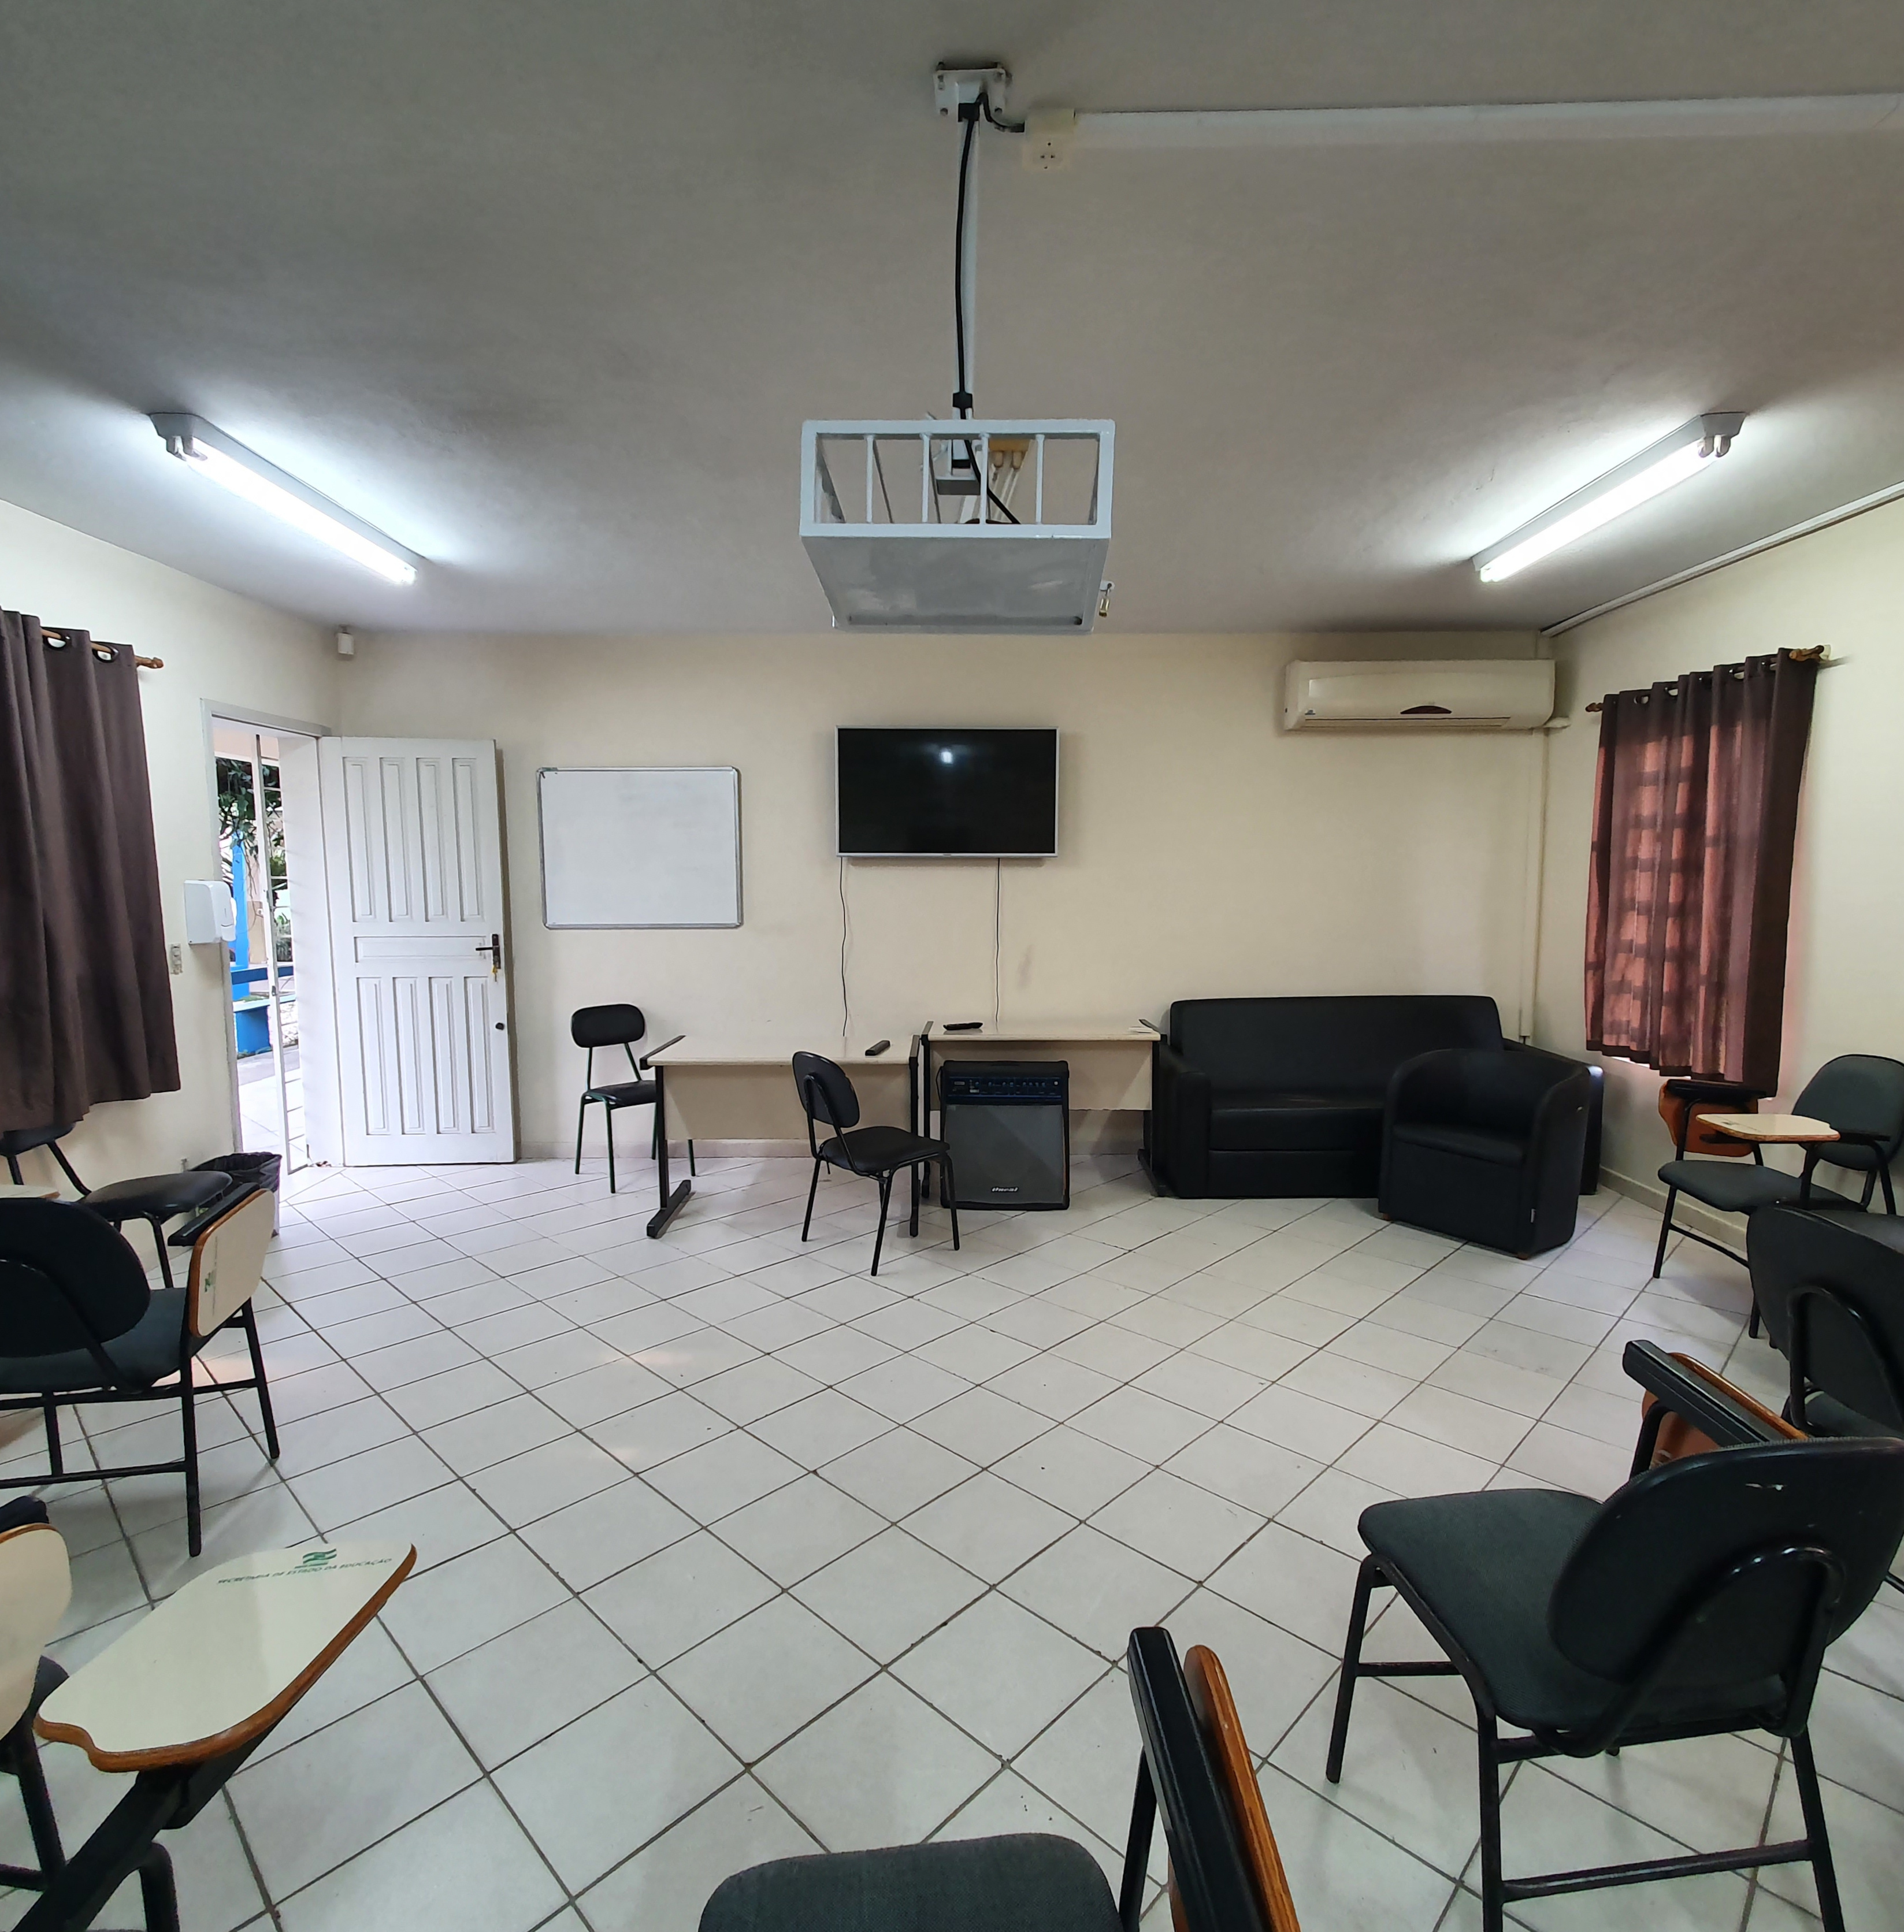
\includegraphics[width=.35\textwidth]{03-elementos/03.2_textual/03.2.1_fig/auditorio01.jpg} 
    \caption{Auditório}
    \label{fig:auditorio}    
\end{wrapfigure}
O auditório tem capacidade para comportar um total 40 pessoas, é equipado com: um televisor de led $40\inch$, caixa de som amplificada multiuso Oneal-OCM modelo 550 de $80\Watt$ de potência rms, um retroprojetor e ar-condicionado.

\section{Biblioteca}
No acervo da Biblioteca encontram-se: livros didáticos de todas as disciplinas, livros de literatura nacional e internacional, almanaques, \acp{DVD} educativos, revistas de assuntos dos mais variádos e jornais. Possui também uma televisão de $32\inch$ a tubo conectada à uma leitora de \ac{DVD}, mesas e cadeiras o suficiente para comportar uma pequena turma de 10 pessoas.
\vfill
\begin{figure}[!ht]
    \begin{center}
        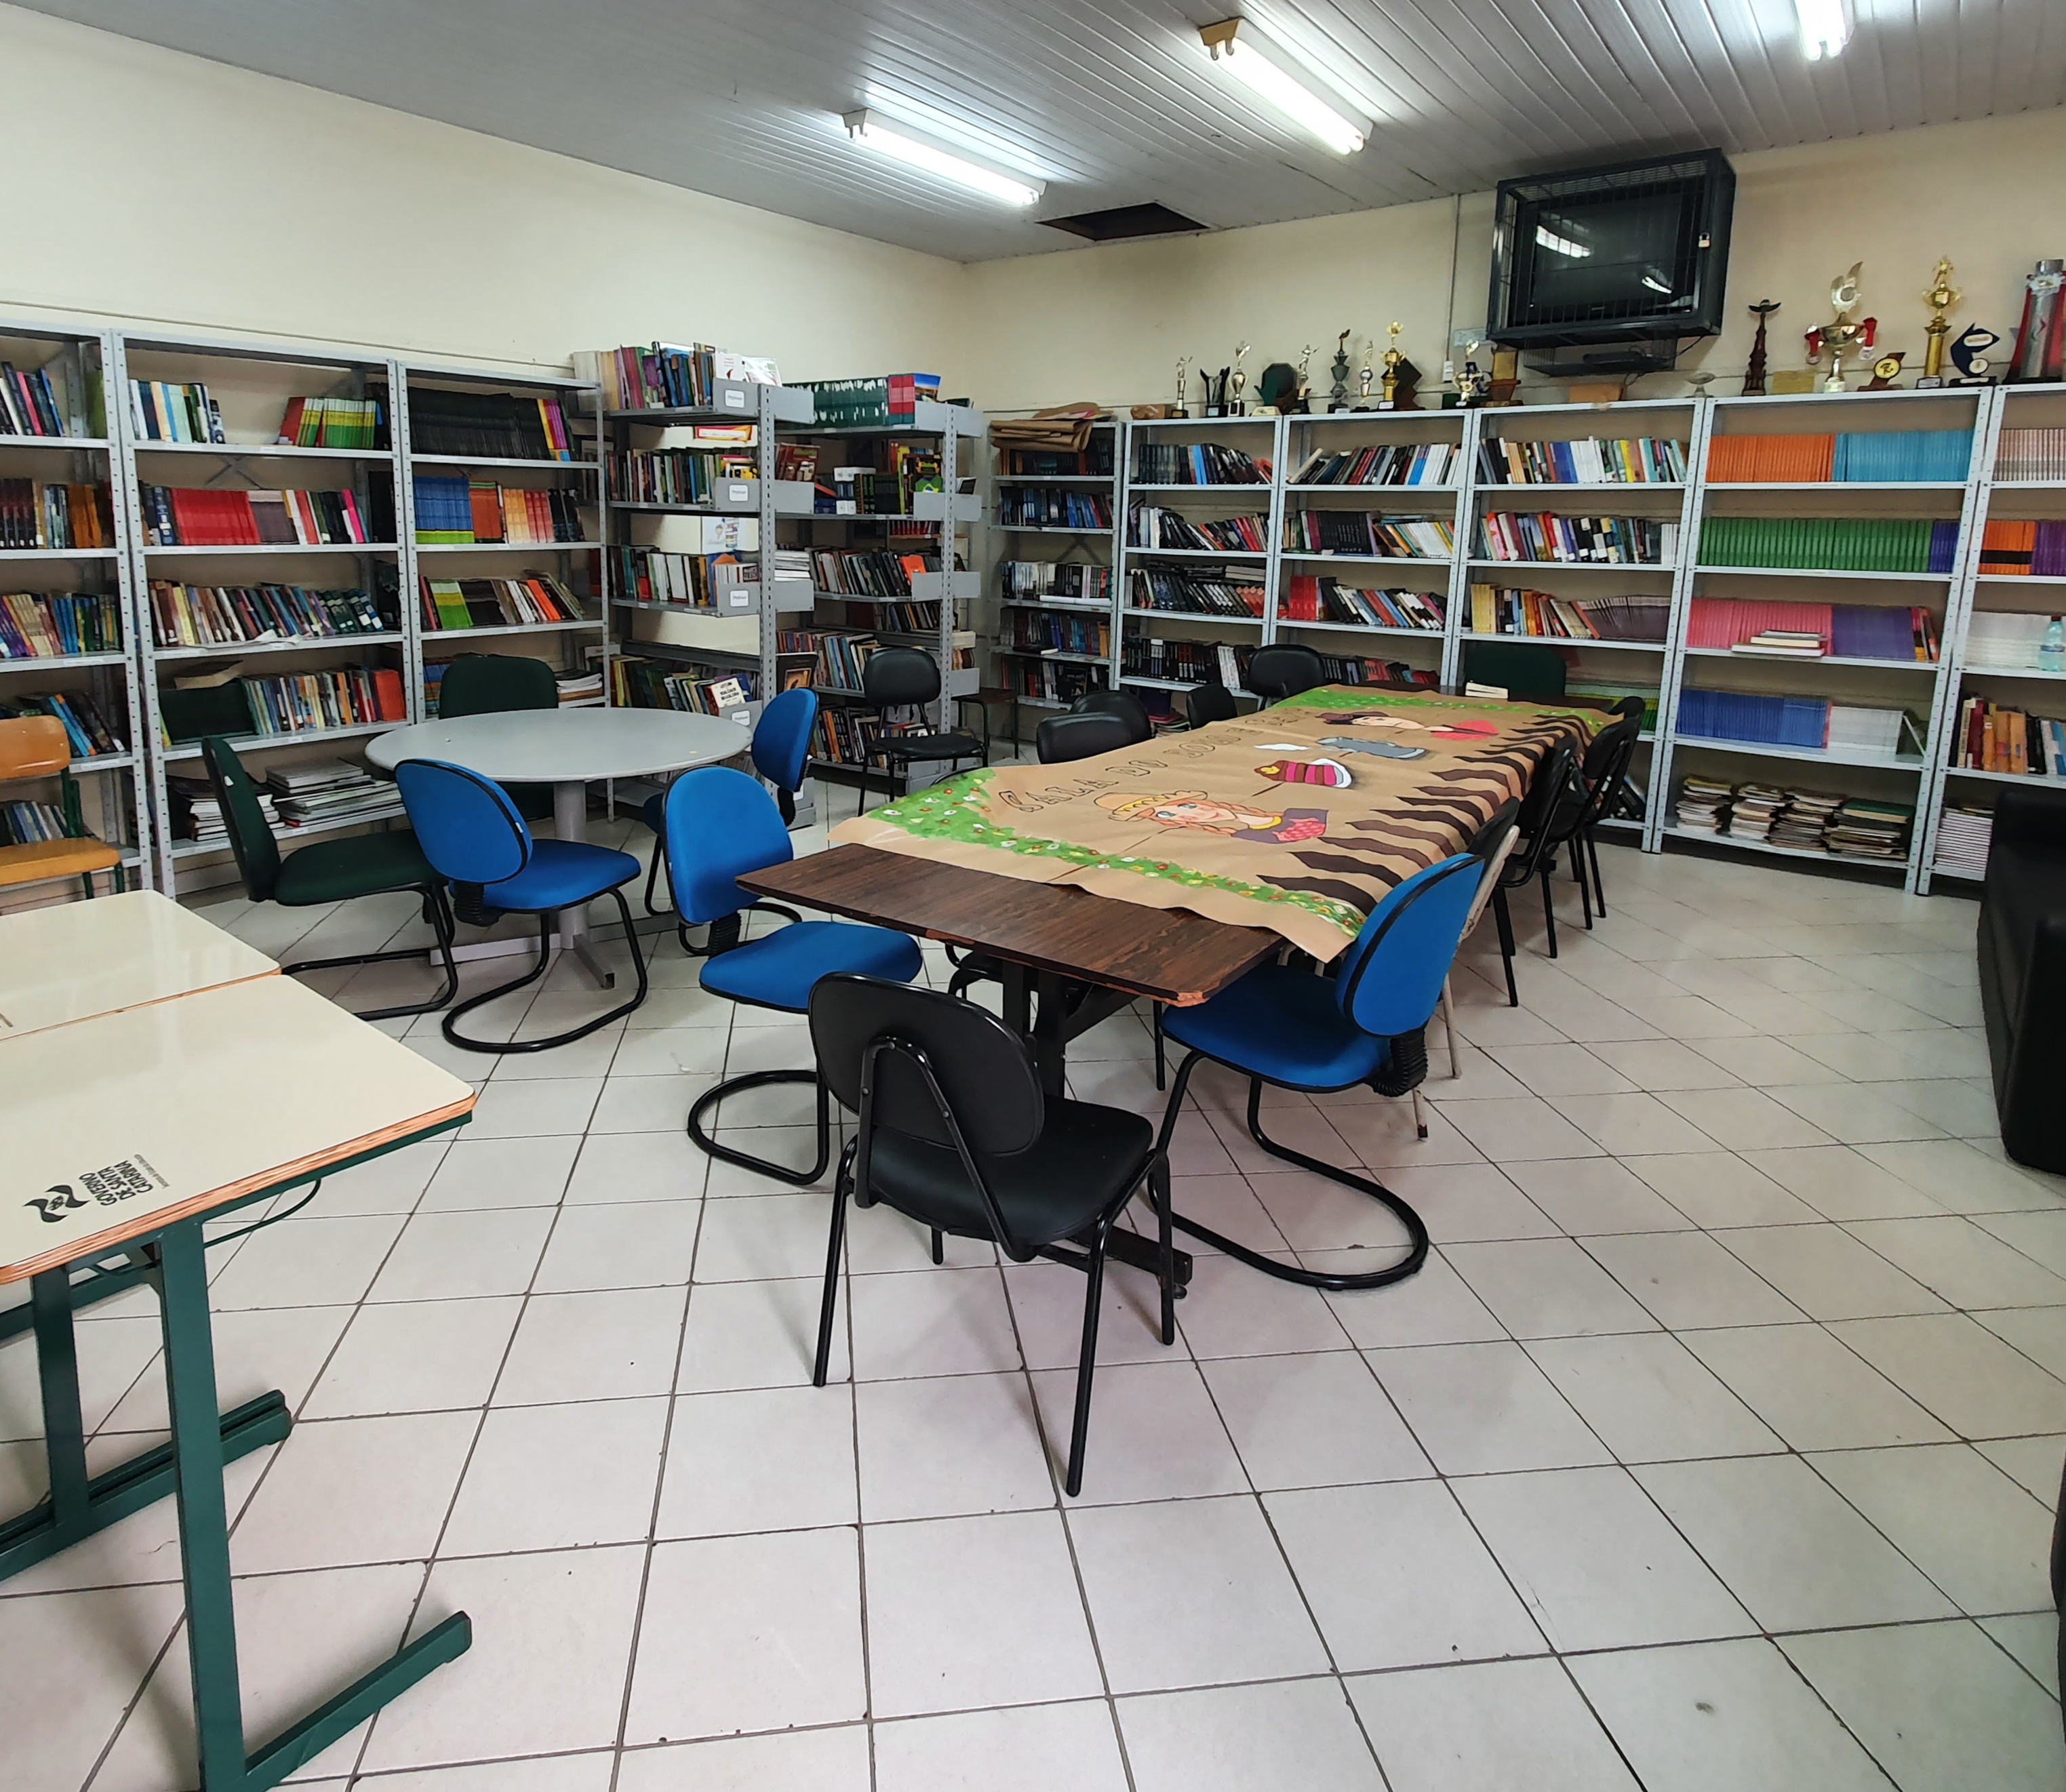
\includegraphics[width=.7\textwidth]{03-elementos/03.2_textual/03.2.1_fig/biblioteca01.jpg}       
        \label{fig:biblioteca}    
        \caption{Biblioteca}
    \end{center}    
\end{figure}



